\chapter{Validation}
\label{chap:validation}

\vspace{-\baselineskip}

%##################################################################################################
\section{Chapter Overview}
%##################################################################################################

In order to evaluate the effectiveness of my approach, I undertook two separate pieces of validation work. The first piece involved quantifying the accuracy of the 3D feature identifiers presented in the previous chapter -- this was done by comparing their output to `gold standard' results produced manually in collaboration with a radiologist. The second piece involved validating the accuracy of my volume calculations (see \S\ref{sec:appendixapps-volumecalc}). To do this, I first manually identified the liver, kidneys and spleen in a number of series and used my program to calculate their volumes in each case. The volume results were then correlated with known weights provided by the radiologist (bearing in mind that the densities of the organs in question are relatively uniform).

Both producing the gold standard results and making inter-result comparisons involved implementing special features for the purpose in \emph{millipede}. For the gold standard production, manual drawing tools were implemented to allow the user to draw round features of interest in the images. To make life easier for the user, the actual drawing was done using a \emph{Bamboo Fun} pen tablet (manufactured by Wacom) -- see Figure~\ref{fig:validation-pentablet-usage} -- although it would also have been possible to use a standard mouse. The inter-result comparisons were implemented as a dialog box allowing the user to compare multi-feature selections on a per-feature basis. The implementation of all the validation-specific features is discussed in Appendix~\ref{chap:appendixval}.

The validation work undertaken here forms an important part of the basis for the following chapter, in which I critically assess all the contributions claimed in the introduction.

%---
\stufigex{height=20cm}{validation/validation-pentablet-usage.png}{A typical user drawing round the right kidney using a `lasso' drawing tool similar to that found in common image-editing programs}{fig:validation-pentablet-usage}{p}
%---

%##################################################################################################
\section{Validation of 3D Feature Identifiers}
%##################################################################################################

To validate my 3D feature identifiers, I undertook four detailed case studies to test how well they worked on sets of slices from different series. An alternative approach of testing them on a larger number of series, but with less detailed individual analysis, would also have been possible, but in my view further work must be done on improving the robustness of the identifiers before such larger-scale validation really makes sense. The aim here is mainly to illustrate some of the areas in which the identifiers currently succeed or fail in order to highlight areas for further work.

For each case study, I produced a `gold standard' result by manually identifying the aorta, kidneys, liver, ribs, spinal canal, spine and spleen using the validation tools described in Appendix~\ref{chap:appendixval}. The resulting features were checked, and corrected where necessary, by Dr Zoe Traill, a Consultant Radiologist at the Churchill Hospital, Oxford. I then identified the same features using the automated multi-feature identifier. To perform a comparison, the gold standard result ($G$) and automated result ($A$) were used to construct three derivative multi-feature selections:
%
\begin{enumerate}
\item $A - G$, which contains the parts of the features that were identified by the automated identifier but should not have been.
\item $G - A$, which contains the parts of the features that were missed by the automated identifier.
\item $A \cap G$, which contains the parts of the features that were correctly identified.
\end{enumerate}
%
These were then used to calculate the Dice similarity coefficient for each feature, as described in \S\ref{sec:appendixval-featurecomparisons}, providing a quantitative measure of the extent to which the automated and gold standard results correspond.

%################################################
\subsection{Series BT-2, Slices $60$--$80$}
%################################################

The first case study was of slices $60$--$80$ from series $2$ of a patient called BT. Side-by-side comparisons of the automated and gold standard results are shown in Table~\ref{tbl:validation-BT-2-60-80} and Figure~\ref{fig:validation-BT-2-60-80}. The identified features can be analysed as follows:
%
\begin{itemize}

\item \textbf{Aorta}. As quantified by the relatively high Dice similarity coefficient of $0.859$ in Table~\ref{tbl:validation-BT-2-60-80}, the automated result for the aorta corresponds fairly well to the gold standard in this case. However, as shown in Figure~\ref{fig:validation-BT-2-60-80}(c), the automated result does flood slightly beyond the aorta itself. Referring back to one of the original slices (see Figure~\ref{fig:validation-BT-2-60-80-aorta-weakedge}), this is because the boundary between the aorta and an adjacent blood vessel (the left renal vein) is quite weak, and the stratified region growing algorithm thus does not know when to stop. This could perhaps be rectified by using level sets instead of region growing. A further problem is that the automated result slightly undersegments the outer boundary, as shown in Figure~\ref{fig:validation-BT-2-60-80}(d). This is primarily an issue with the original segmentation produced when constructing the partition forest.

\item \textbf{Kidneys}. Only the right kidney was relevant in this case, as the left kidney had been entirely overtaken by a huge tumour. As indicated by the high Dice similarity coefficient of $0.949$, the automated result for the kidney that was present was good. The minor discrepancies are primarily due to the automated identifier slightly oversegmenting the region around the renal pelvis.

\item \textbf{Liver}. Given the relative complexity of liver identification compared to identifying other features, the automated result in this case is fairly good, with a Dice similarity coefficient of $0.890$. However, Figure~\ref{fig:validation-BT-2-60-80}(d) illustrates that the lateral segment of the left lobe is clearly missed. This is due to the current approach doing only single-seed region growing -- in the slices chosen, the lateral segment of the left lobe and the rest of the liver are not connected (see Figure~\ref{fig:validation-BT-2-60-80-liver-disconnected}), so the algorithm finds one part of the liver but not the other. This could be rectified in this case by using multi-seed region growing, although some care would need to be taken over choosing appropriate seeds to make sure that other features in the area were not mistakenly identified as being part of the liver. A further problem with the automated liver result is that it floods beyond the boundary of the liver in the direction of the aorta (see Figure~\ref{fig:validation-BT-2-60-80}(c)). As with the aorta result, this is due to a weak boundary, and a level sets approach might be more effective.

\item \textbf{Ribs}. The ribs are identified reasonably well in this case, with a Dice similarity coefficient of $0.773$. The main source of inaccuracy, as can be seen in Figures~\ref{fig:validation-BT-2-60-80}(c) and (d), is that the automated identifier has incorrectly identified the top-most ribs as spine (hence Table~\ref{tbl:validation-BT-2-60-80} contains a high $G - A$ value for ribs). As was mentioned in the previous chapter, this is a known problem with the current ribs identifier, in that it deliberately avoids marking as rib anything that has already been marked as spine, thus giving priority to the spine where there is a conflict between the two. This is considered a suitable area for further work.

\item \textbf{Spinal Canal}. The spinal canal identifier works fairly well here, with a Dice similarity coefficient of $0.840$. The number of missed voxels ($309$) is relatively small in comparison to the overall size of the canal; the more significant issue is that the spinal canal has been somewhat oversegmented, hence the slightly high value for $A - G$ in this case. The major reason for this is that the spinal canal identifier currently works by filtering for suitable branch nodes (see Listing~\ref{code:featureid-3d-spinalcanalidentification}), and this relies on regions in the partition forest being exactly the right shape. For the spinal canal, this is roughly the case, which is why the approach works reasonably well. However, waterfall hierarchies converge relatively quickly (i.e.~the number of nodes in each layer decreases rapidly as we go towards the top of the forest) -- by the time enough smaller regions inside the spinal column have been merged to form a suitable region that can be identified as the spinal canal, surrounding regions inside the spinal column have usually been dragged in as well, ultimately leading to oversegmentation of the spinal canal (see Figure~\ref{fig:validation-BT-2-60-80-spinalcanal-oversegmentation}). A possible way of improving the situation would be to use the outer contour of the existing result (which is generally fairly good) to initialise a level set method that could be used to refine the boundary.

\item \textbf{Spine}. As witnessed by a high Dice similarity coefficient of $0.926$, the spine identifier produces relatively good results in this case. However, as mentioned earlier, there is a tendency for the spine to be oversegmented at the expense of the ribs when there is a conflict between them. Furthermore, as can be seen in Figure~\ref{fig:validation-BT-2-60-80}(d), the automated identifier often misses the \emph{transverse processes} of the spine (that is, the pieces that protrude to the left and right of the main spinal column). This is primarily because it currently uses a branch node filtering approach (see Listing~\ref{code:featureid-3d-spineidentification}), and the processes are not generally merged into the main spine region during forest construction (see Figure~\ref{fig:validation-BT-2-60-80-spine-transverseprocesses}). Since the primary aim of the spine identifier in this thesis is to provide a landmark that can be used when identifying other organs, this is not considered to be a major issue for our purposes here, but further work could be done to improve the identifier in this regard.

\item \textbf{Spleen}. Despite the relatively incipient nature of the spleen identifier, it performs in some ways surprisingly well on the BT-2 case study, with a Dice similarity coefficient of $0.853$. At present, however, the identifier undersegments the spleen because it accepts the initial spleen seed as is, without attempting to grow a full spleen feature from it (see Listing~\ref{code:featureid-3d-spleenidentification}). Ultimately, it may be sensible to use the spleen seed to initialise a level sets approach, but this is a subject for further work.

\end{itemize}

%---
\begin{table}[p]
\begin{center}
\begin{tabular}{c|cccccc}
\footnotesize \textbf{Feature} & \footnotesize \textbf{Automated (A)} & \footnotesize \textbf{Gold (G)} & \footnotesize \textbf{A -- G} & \footnotesize \textbf{G -- A} & \footnotesize \textbf{A $\cap$ G} & \footnotesize \textbf{Dice} \\
\hline
\footnotesize Aorta & \footnotesize 13940 & \footnotesize 13973 & \footnotesize 1949 & \footnotesize 1982 & \footnotesize 11991 & \footnotesize 0.859 \\
\footnotesize Kidneys & \footnotesize 72142 & \footnotesize 73715 & \footnotesize 2915 & \footnotesize 4488 & \footnotesize 69227 & \footnotesize 0.949 \\
\footnotesize Liver & \footnotesize 180156 & \footnotesize 180693 & \footnotesize 19624 & \footnotesize 20161 & \footnotesize 160532 & \footnotesize 0.890 \\
\footnotesize Ribs & \footnotesize 22787 & \footnotesize 31125 & \footnotesize 1942 & \footnotesize 10280 & \footnotesize 20845 & \footnotesize 0.773 \\
\footnotesize Spinal Canal & \footnotesize 14451 & \footnotesize 11002 & \footnotesize 3758 & \footnotesize 309 & \footnotesize 10693 & \footnotesize 0.840 \\
\footnotesize Spine & \footnotesize 111889 & \footnotesize 113385 & \footnotesize 7634 & \footnotesize 9130 & \footnotesize 104255 & \footnotesize 0.926 \\
\footnotesize Spleen & \footnotesize 11841 & \footnotesize 15077 & \footnotesize 359 & \footnotesize 3595 & \footnotesize 11482 & \footnotesize 0.853 \\
\end{tabular}
\end{center}
\caption{A numeric comparison of the automated and gold standard results for the BT-2-60-80 feature identification case study. (All entries except those for the similarity coefficient are in voxels.)}
\label{tbl:validation-BT-2-60-80}
\end{table}
%---

%---
\begin{stusubfig}{p}
	\subfigure[Automated Result ($A$)]
	{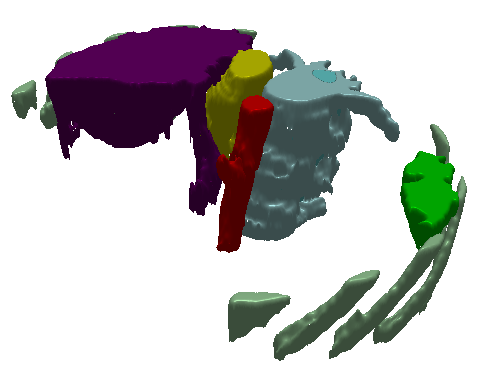
\includegraphics[width=.45\linewidth]{validation/validation-BT-2-60-80-target.png}}%
	%
	\hspace{4mm}%
	%
	\subfigure[Gold Standard Result ($G$)]
	{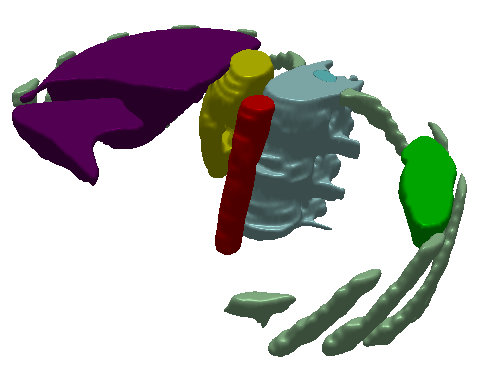
\includegraphics[width=.45\linewidth]{validation/validation-BT-2-60-80-goldstandard.png}}%
	%
	\\
	%
	\subfigure[$A - G$]
	{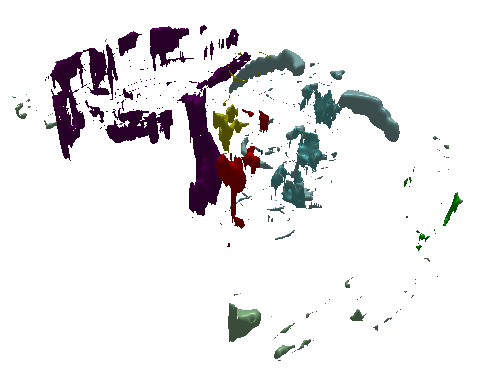
\includegraphics[width=.45\linewidth]{validation/validation-BT-2-60-80-TminusG.png}}%
	%
	\hspace{4mm}%
	%
	\subfigure[$G - A$]
	{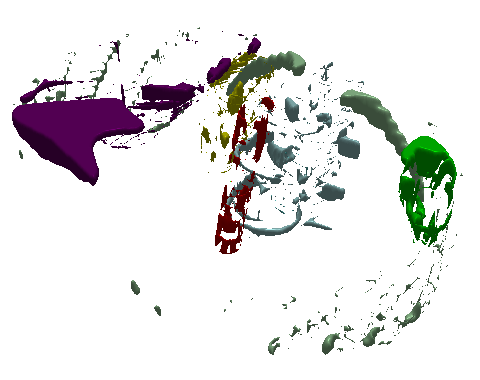
\includegraphics[width=.45\linewidth]{validation/validation-BT-2-60-80-GminusT.png}}%
\caption{A visual comparison of the automated and gold standard results for the BT-2-60-80 feature identification case study}
\label{fig:validation-BT-2-60-80}
\end{stusubfig}
%---

%---
\stufigex{height=8cm}{validation/validation-BT-2-60-80-aorta-weakedge-labelled.png}{The aorta identifier can flood into adjacent blood vessels, such as the left renal vein, due to weak boundaries in the original images}{fig:validation-BT-2-60-80-aorta-weakedge}{p}
%---

%---
\stufigex{height=8cm}{validation/validation-BT-2-60-80-liver-disconnected-labelled.png}{The liver identifier misses the lateral segment of the left lobe in the BT-2 case study because it is not connected to the rest of the liver in the slices chosen}{fig:validation-BT-2-60-80-liver-disconnected}{p}
%---

%---
\stufigex{height=8cm}{validation/validation-BT-2-60-80-spinalcanal-oversegmentation.png}{The spinal canal tends to be slightly oversegmented, with surrounding voxels, such as those marked in blue, identified when they should not be}{fig:validation-BT-2-60-80-spinalcanal-oversegmentation}{p}
%---

%---
\begin{stusubfig}{p}
	\subfigure[]
	{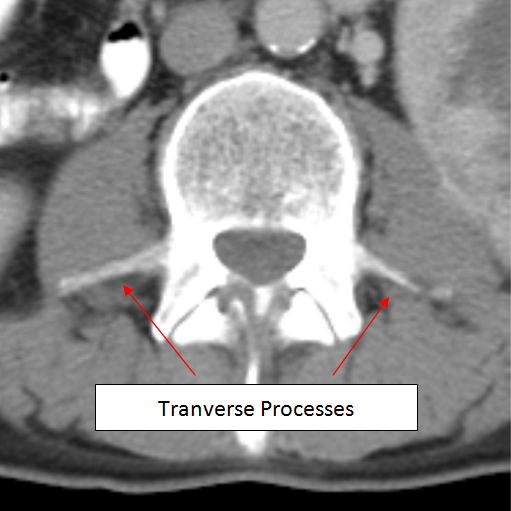
\includegraphics[width=.45\linewidth]{validation/validation-BT-2-60-80-spine-transverseprocesses-a-labelled.png}}%
	%
	\hspace{4mm}%
	%
	\subfigure[]
	{
\includegraphics[width=.45\linewidth]{validation/validation-BT-2-60-80-spine-transverseprocesses-b.png}}%
\caption{The spine identifier misses the transverse processes of the spine (a) in the BT-2 case study, because the hierarchical segmentation process does not merge them into the main spine region (b)}
\label{fig:validation-BT-2-60-80-spine-transverseprocesses}
\end{stusubfig}
%---

\afterpage{\clearpage}
\newpage

%################################################
\subsection{Series SD-2, Slices $70$--$90$}
%################################################

\iffalse

Aorta

- Fairly good (Dice = 0.811)
- Floods out into a neighbouring blood vessel somewhat -- which one? same reason as for BT-2?

Kidneys

- Only one -- why? (can't remember)
- Good (Dice = 0.931)
- Automated result not quite as smooth -- why? (primarily an issue with the underlying segmentation)

Liver

- Good (Dice = 0.932)
- Doesn't miss a major part of the liver this time, because it's connected in the slices chosen
- Floods out towards the aorta -- why? (probably a weak edge)

Ribs

- Fairly good (Dice = 0.819)
- Picks up an erroneous bit which isn't a rib -- why? (probably because very bright in the image)
- Misses the odd bit which is a rib -- why? (check differences on scans)

Spinal Canal

- Fairly good (Dice = 0.862)
- Somewhat oversegmented -- for the same reasons mentioned for BT-2

Spine

- Good (Dice = 0.965), partly on account of this patient's notably high bone density
- Only minor differences, largely due to slight subjectivity of gold standard

Spleen

- Fairly good (Dice = 0.874)
- The automated result has missed a lot of the spleen -- why? (probably because I'm only finding a seed and not then flooding out from it)
- The automated result contains a lot of holes -- why? (probably because I'm not currently doing any hole filling)

\fi

TODO

%---
\begin{table}[p]
\begin{center}
\begin{tabular}{c|cccccc}
\footnotesize \textbf{Feature} & \footnotesize \textbf{Automated (A)} & \footnotesize \textbf{Gold (G)} & \footnotesize \textbf{A -- G} & \footnotesize \textbf{G -- A} & \footnotesize \textbf{A $\cap$ G} & \footnotesize \textbf{Dice} \\
\hline
\footnotesize Aorta & \footnotesize 12799 & \footnotesize 9848 & \footnotesize 3619 & \footnotesize 668 & \footnotesize 9180 & \footnotesize 0.811 \\
\footnotesize Kidneys & \footnotesize 93853 & \footnotesize 91324 & \footnotesize 7671 & \footnotesize 5142 & \footnotesize 86182 & \footnotesize 0.931 \\
\footnotesize Liver & \footnotesize 254945 & \footnotesize 231766 & \footnotesize 28156 & \footnotesize 4977 & \footnotesize 226789 & \footnotesize 0.932 \\
\footnotesize Ribs & \footnotesize 10331 & \footnotesize 10097 & \footnotesize 1962 & \footnotesize 1728 & \footnotesize 8369 & \footnotesize 0.819 \\
\footnotesize Spinal Canal & \footnotesize 15163 & \footnotesize 11655 & \footnotesize 3609 & \footnotesize 101 & \footnotesize 11554 & \footnotesize 0.862 \\
\footnotesize Spine & \footnotesize 84757 & \footnotesize 85430 & \footnotesize 2624 & \footnotesize 3297 & \footnotesize 82133 & \footnotesize 0.965 \\
\footnotesize Spleen & \footnotesize 46129 & \footnotesize 55049 & \footnotesize 1922 & \footnotesize 10842 & \footnotesize 44207 & \footnotesize 0.874 \\
\end{tabular}
\end{center}
\caption{A numeric comparison of the automated and gold standard results for the SD-2-70-90 feature identification case study. (All entries except those for the similarity coefficient are in voxels.)}
\label{tbl:validation-SD-2-70-90}
\end{table}
%---

%---
\begin{stusubfig}{p}
	\subfigure[Automated Result ($A$)]
	{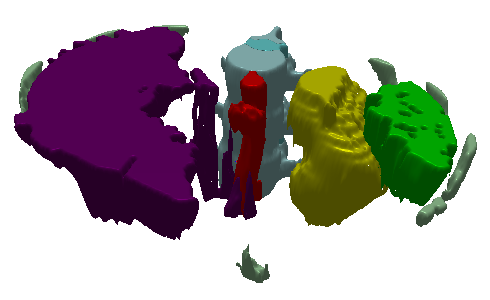
\includegraphics[width=.45\linewidth]{validation/validation-SD-2-70-90-target.png}}%
	%
	\hspace{4mm}%
	%
	\subfigure[Gold Standard Result ($G$)]
	{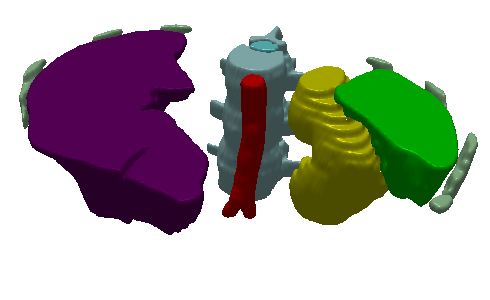
\includegraphics[width=.45\linewidth]{validation/validation-SD-2-70-90-goldstandard.png}}%
	%
	\\
	%
	\subfigure[$A - G$]
	{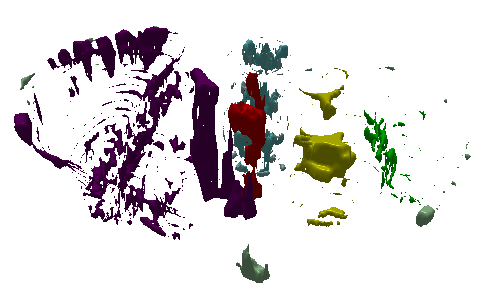
\includegraphics[width=.45\linewidth]{validation/validation-SD-2-70-90-TminusG.png}}%
	%
	\hspace{4mm}%
	%
	\subfigure[$G - A$]
	{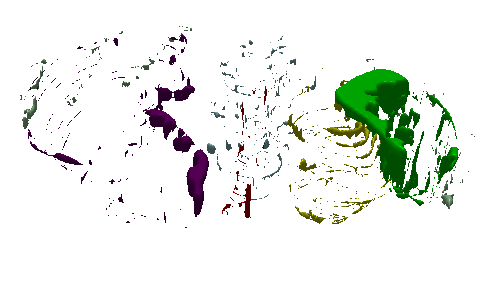
\includegraphics[width=.45\linewidth]{validation/validation-SD-2-70-90-GminusT.png}}%
\caption{A visual comparison of the automated and gold standard results for the SD-2-70-90 feature identification case study}
\label{fig:validation-SD-2-70-90}
\end{stusubfig}
%---

\afterpage{\clearpage}
\newpage

%################################################
\subsection{Series MC-2, Slices $110$--$130$}
%################################################

\iffalse

Aorta

- Good (Dice = 0.908)
- Minor differences -- why? (primarily a result of the underlying segmentation)
- Overlapped by the liver, which has flooded out too far
  - The "easy" way to fix this is to unidentify as liver anything also marked as aorta, and then to find the connected components of the remaining liver bits and only keep sensible ones -- but that doesn't solve the problem in the general case

Kidneys

- Fairly good (Dice = 0.906)
- Flooded out a bit too far on the left kidney -- why? (check scans)
- The automated result is a bit smoother than the gold standard (not surprising, the slices are 5mm thick and the Laplacian smoothing is not perfect)

Liver

- Fairly good (Dice = 0.848)
- Flooded out much too far towards the aorta (completely overlapping it) -- why? (probably a weak edge)
- General outline isn't too bad
- Missed medial segment of left lobe -- why? (check scans)

Ribs

- Fairly good (Dice = 0.816)
- The automated result misses internal bits of ribs -- why?

Spinal Canal

- Good (Dice = 0.933)
- As ever, the automated result is slightly oversegmented -- see discussion for BT-2

Spine

- Good (Dice = 0.947)
- Minor differences are probably due to slight subjectivity of the gold standard (but check scans)

Spleen

- Fairly good (Dice = 0.898)
- As with SD-2, a certain amount of the spleen has been missed because not doing region flooding yet
- As with SD-2, contains a number of holes because not doing hole filling yet

\fi

TODO

%---
\begin{table}[p]
\begin{center}
\begin{tabular}{c|cccccc}
\footnotesize \textbf{Feature} & \footnotesize \textbf{Automated (A)} & \footnotesize \textbf{Gold (G)} & \footnotesize \textbf{A -- G} & \footnotesize \textbf{G -- A} & \footnotesize \textbf{A $\cap$ G} & \footnotesize \textbf{Dice} \\
\hline
\footnotesize Aorta & \footnotesize 15799 & \footnotesize 15036 & \footnotesize 1805 & \footnotesize 1042 & \footnotesize 13994 & \footnotesize 0.908 \\
\footnotesize Kidneys & \footnotesize 148065 & \footnotesize 137416 & \footnotesize 18698 & \footnotesize 8049 & \footnotesize 129367 & \footnotesize 0.906 \\
\footnotesize Liver & \footnotesize 492435 & \footnotesize 413475 & \footnotesize 108454 & \footnotesize 29494 & \footnotesize 383981 & \footnotesize 0.848 \\
\footnotesize Ribs & \footnotesize 33626 & \footnotesize 42708 & \footnotesize 2483 & \footnotesize 11565 & \footnotesize 31143 & \footnotesize 0.816 \\
\footnotesize Spinal Canal & \footnotesize 9924 & \footnotesize 9087 & \footnotesize 1054 & \footnotesize 217 & \footnotesize 8870 & \footnotesize 0.933 \\
\footnotesize Spine & \footnotesize 81483 & \footnotesize 79453 & \footnotesize 5247 & \footnotesize 3217 & \footnotesize 76236 & \footnotesize 0.947 \\
\footnotesize Spleen & \footnotesize 32048 & \footnotesize 36537 & \footnotesize 1240 & \footnotesize 5729 & \footnotesize 30808 & \footnotesize 0.898 \\
\end{tabular}
\end{center}
\caption{A numeric comparison of the automated and gold standard results for the MC-2-110-130 feature identification case study. (All entries except those for the similarity coefficient are in voxels.)}
\label{tbl:validation-MC-2-110-130}
\end{table}
%---

%---
\begin{stusubfig}{p}
	\subfigure[Gold Standard Result]
	{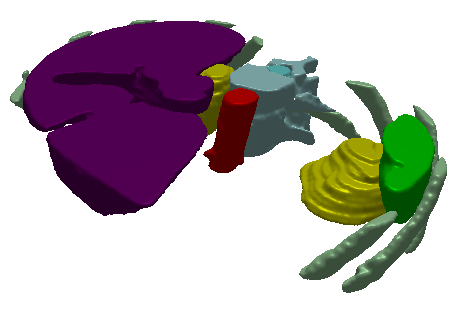
\includegraphics[width=.45\linewidth]{validation/validation-MC-2-110-130-goldstandard.png}}%
	%
	\hspace{4mm}%
	%
	\subfigure[Automated Result]
	{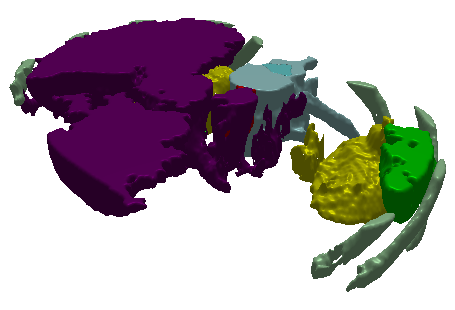
\includegraphics[width=.45\linewidth]{validation/validation-MC-2-110-130-target.png}}%
	%
	\hspace{4mm}%
	%
	\subfigure[Automated Result (excluding liver)]
	{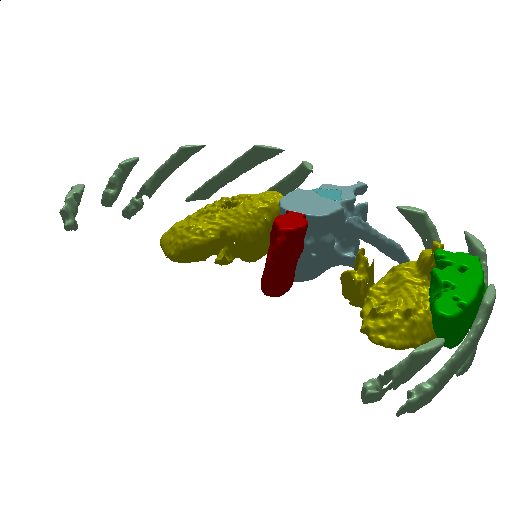
\includegraphics[width=.45\linewidth]{validation/validation-MC-2-110-130-target-noliver.png}}%
\caption{TODO}
\label{fig:validation-MC-2-110-130}
\end{stusubfig}
%---

\afterpage{\clearpage}
\newpage

%################################################
\subsection{Series EB-2, Slices $60$--$80$}
%################################################

\iffalse

Aorta

- Fairly good (Dice = 0.849)
- Automated result sticks out too far at the front -- why?
- Automated result is also missing bits in places -- where, and why? (check scans)

Kidneys

- Right kidney is good (Dice = 0.932)
- Left kidney is completely missed -- why? (primarily because of the tumour)
- Minor differences for right kidney are probably due to slight subjectivity of gold standard

Liver

- Good (0.948)
- Missing small bits of the left lobe -- why? (primarily because they're not connected in the slices chosen)
- Missing bits at the back -- why? (check scans)

Ribs

- Poor (Dice = 0.488)
- Segmenting lots of bits which aren't rib -- why? (probably because there are very bright bits on the images)

Spinal Canal

- Fairly good (Dice = 0.856)
- Again, somewhat oversegmented -- same reasons as for other series

Spine

- Good (Dice = 0.925)
- Automated result missing some of the bits sticking out -- why? (primarily because using branch node filtering instead of region growing, but also because some of the bits may be quite dark)
- Also segmenting bits it shouldn't -- which bits? (check scans)

Spleen

- Completely missed -- why? (check scans)

\fi

TODO (the left kidney is missed due to a tumour; the spleen is missed because there's not enough of it in the slices chosen (check this); the ribs are oversegmented because there are lots of unusually bright non-rib bits in EB-2)

%---
\begin{table}[p]
\begin{center}
\begin{tabular}{c|cccccc}
\footnotesize \textbf{Feature} & \footnotesize \textbf{Automated (A)} & \footnotesize \textbf{Gold (G)} & \footnotesize \textbf{A -- G} & \footnotesize \textbf{G -- A} & \footnotesize \textbf{A $\cap$ G} & \footnotesize \textbf{Dice} \\
\hline
\footnotesize Aorta & \footnotesize 10365 & \footnotesize 9416 & \footnotesize 1969 & \footnotesize 1020 & \footnotesize 8396 & \footnotesize 0.849 \\
\footnotesize Kidney (Right) & \footnotesize 47444 & \footnotesize 46918 & \footnotesize 3461 & \footnotesize 2935 & \footnotesize 43983 & \footnotesize 0.932 \\
\footnotesize Kidney (Left) & \footnotesize 0 & \footnotesize 36874 & \footnotesize 0 & \footnotesize 36874 & \footnotesize 0 & \footnotesize 0.000 \\
\footnotesize Liver & \footnotesize 160978 & \footnotesize 164834 & \footnotesize 6592 & \footnotesize 10448 & \footnotesize 154386 & \footnotesize 0.948 \\
\footnotesize Ribs & \footnotesize 10256 & \footnotesize 4959 & \footnotesize 6542 & \footnotesize 1245 & \footnotesize 3714 & \footnotesize 0.488 \\
\footnotesize Spinal Canal & \footnotesize 12387 & \footnotesize 9645 & \footnotesize 2958 & \footnotesize 216 & \footnotesize 9429 & \footnotesize 0.856 \\
\footnotesize Spine & \footnotesize 82721 & \footnotesize 85490 & \footnotesize 4946 & \footnotesize 7715 & \footnotesize 77775 & \footnotesize 0.925 \\
\footnotesize Spleen & \footnotesize 0 & \footnotesize 20179 & \footnotesize 0 & \footnotesize 20179 & \footnotesize 0 & \footnotesize 0.000 \\
\end{tabular}
\end{center}
\caption{A numeric comparison of the automated and gold standard results for the EB-2-60-80 feature identification case study. (All entries except those for the similarity coefficient are in voxels.)}
\label{tbl:validation-EB-2-60-80}
\end{table}
%---

%---
\begin{stusubfig}{p}
	\subfigure[Automated Result ($A$)]
	{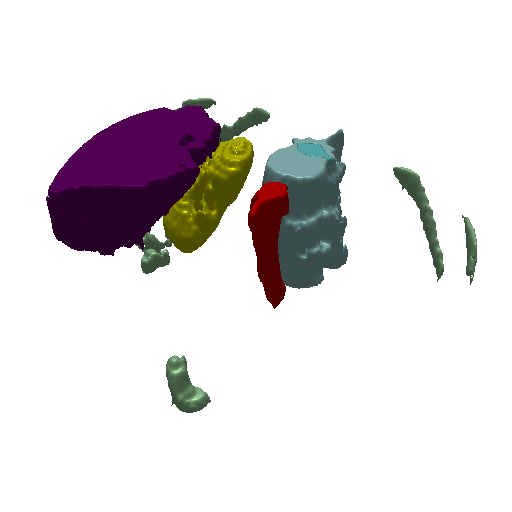
\includegraphics[width=.45\linewidth]{validation/validation-EB-2-60-80-target.png}}%
	%
	\hspace{4mm}%
	%
	\subfigure[Gold Standard Result ($G$)]
	{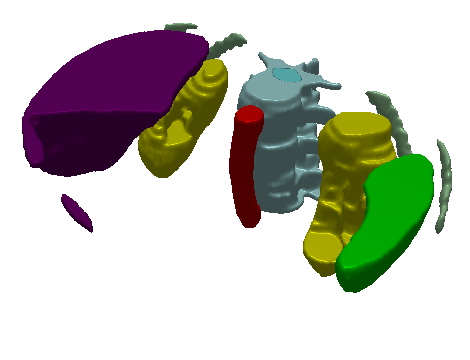
\includegraphics[width=.45\linewidth]{validation/validation-EB-2-60-80-goldstandard.png}}%
	%
	\\
	%
	\subfigure[$A - G$]
	{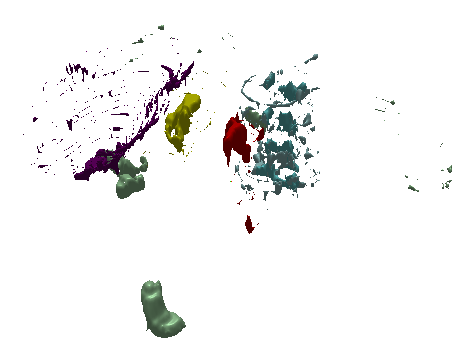
\includegraphics[width=.45\linewidth]{validation/validation-EB-2-60-80-TminusG.png}}%
	%
	\hspace{4mm}%
	%
	\subfigure[$G - A$]
	{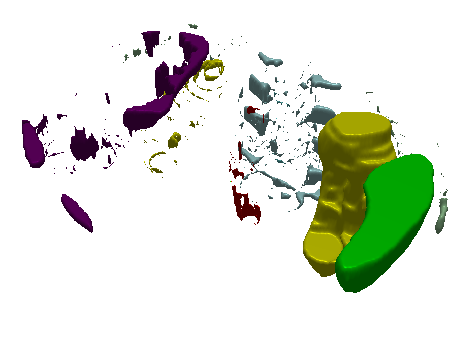
\includegraphics[width=.45\linewidth]{validation/validation-EB-2-60-80-GminusT.png}}%
\caption{A visual comparison of the automated and gold standard results for the EB-2-60-80 feature identification case study}
\label{fig:validation-EB-2-60-80}
\end{stusubfig}
%---

\afterpage{\clearpage}
\newpage

%##################################################################################################
\section{Validation of Volume Calculations}
%##################################################################################################

The ideal way to validate my volume calculations would have been to correlate them with real-world volumes calculated independently by the medics, but unfortunately these were not available. However, I was able to obtain the \emph{masses} of patients' organs calculated post-mortem as part of a study into the feasibility of performing virtual autopsies \cite{?}. These provided a reasonable (if not perfect) substitute for the volumes, since the major soft-tissue organs have known, and roughly uniform, densities (this is why they appear homogeneous on CT scans, since the Hounsfield scale used for CT images measures radiodensity). In conjunction with Dr Zoe Traill, the radiologist, it was therefore decided to focus on four different features -- the left and right kidneys, liver and spleen. I drew round these features in $19$ series ($740$ slices in total), with the results being checked, and corrected where necessary, by Dr Traill. The calculated volumes (in $\mathit{cm}^3$) resulting from this manual feature identification process are shown in Table~\ref{tbl:validation-volcalc}, alongside the corresponding masses (in $g$) calculated during the autopsies.

When drawing round the features, I was careful to include any cysts on the kidneys, as Dr Traill asserted that these would have been included when weighing the organs during the autopsy. In one case -- for the right kidney of patient OX46 -- this significantly affected the result, due to a large ($80\mathit{mm}$ diameter) cyst being included in the volume calculation whilst not appearing to affect the mass in a similar way. It was hypothesised that this may have been due to the cyst bursting before the kidney was weighed. For that reason, the result in question was specifically excluded as an outlier.

As shown in Table~$3$ of \cite{woodard86}, the accepted densities of the kidneys, liver and spleen are respectively $1050 \; \mathit{kg} \; m^{-3} = 1.05 \; g \; \mathit{cm}^{-3}$, $1050$--$1070 \; \mathit{kg} \; m^{-3} = 1.05$--$1.07 \; g \; \mathit{cm}^{-3}$ and $1060 \; \mathit{kg} m^{-3} = 1.06 \; g \; \mathit{cm}^{-3}$. The validation method involved graphing volumes (on the $x$ axis) against masses (on the $y$ axis) for each feature. Given the uniform densities of the organs involved, each graph was expected to be linear. It was therefore possible to fit a linear regression line in each case, whose gradient was expected to be reasonably close to the accepted density of the feature in $g \; \mathit{cm}^{-3}$.

As illustrated by the graphs in Figures~\ref{fig:validation-volcalc-leftkidney} to \ref{fig:validation-volcalc-spleen}, these expectations were largely borne out. To $2$ decimal places, the densities (in $g \; \mathit{cm}^{-3}$) of the organs as calculated from the linear regression lines on the graphs were $1.15$ for the left kidney, $1.12$ for the right kidney, $1.07$ for the liver and $1.14$ for the spleen. These were considered to be reasonably good results, especially for the liver.

There are number of sources of potential inaccuracy which can explain the discrepancies between the calculated densities and the accepted densities provided in \cite{woodard86}:
%
\begin{enumerate}

\item At the volume calculation end, it is sometimes very difficult even for an experienced radiologist to be certain of the precise boundary round a given organ -- indeed, subjectivity between different radiologists is a known issue in segmentation validation \cite{?}. Since the series used for validation here were all imaged post-mortem (and thus without the benefit of a contrast agent), being certain of the precise boundaries was more than usually difficult for some patients in this case.

\item At the mass calculation end, the precise masses calculated depend on the way in which the organs are resected during the autopsies. It is highly unlikely that anyone performing an organ resection would be able to attain an organ boundary that precisely matched that shown on the CT scan.

%(Indeed, having witnessed an operation in the past and seen some of the difficulties involved in surgical procedures, I find it encouraging that the results match up as closely as they do in this case.)

\item In many of the series being validated, cysts were present on one or both kidneys. Depending on the type of cyst involved, these were either more or less dense than the adjoining kidney tissue, thus affecting the uniform density assumption. In most cases, however, these cysts were not large enough to significantly affect the results.

\end{enumerate}
%
Given the above factors affecting the results, I consider that my volume calculation method itself is relatively accurate. From a medical perspective, this suggests that it may be possible to predict the masses of organs by using volumes calculated from CT scans. This could be useful in cases where it is considered undesirable to perform an autopsy.

%---
\begin{landscape}
\begin{table}[p]
\footnotesize
\begin{center}
\begin{tabular}{c|rrc|rrc|rr|rr}
\textbf{Patient} & \multicolumn{3}{|c|}{\textbf{Left Kidney}} & \multicolumn{3}{|c|}{\textbf{Right Kidney}} & \multicolumn{2}{|c|}{\textbf{Liver}} & \multicolumn{2}{|c}{\textbf{Spleen}} \\
& \emph{Mass} ($g$) & \emph{Vol.} ($\mathit{cm}^3$) & \emph{Cysts} $> 5\mathit{mm}$ & \emph{Mass} ($g$) & \emph{Vol.} ($\mathit{cm}^3$) & \emph{Cysts} $> 5\mathit{mm}$ & \emph{Mass} ($g$) & \emph{Vol.} ($\mathit{cm}^3$) & \emph{Mass} ($g$) & \emph{Vol.} ($\mathit{cm}^3$) \\
\hline
\hline
OX25 & 120 &  96.116 &            --- & 110 &  96.044 &                            --- & 1680 & 1468.657 & 110 & 105.568 \\
OX26 & 190 & 173.155 &            --- & 190 & 175.411 &                            --- & 1790 & 1752.384 &  40 &  32.879 \\
OX27 &  80 &  74.897 &              6 &  85 &  84.300 &                             12 & 1370 & 1156.192 & 140 & 121.837 \\
OX29 & 110 & 106.566 &            --- &  90 &  94.306 &                            --- & 1380 & 1323.991 & 170 & 121.665 \\
OX30 & 120 & 126.524 &         28, 27 & 120 & 113.079 &                              9 & 1819 & 1662.805 & 180 & 158.506 \\
OX31 & 200 & 175.163 &             14 & 170 & 153.155 &                            --- & 2120 & 1972.002 & 110 &  98.132 \\
OX33 & 120 & 111.776 &         12, 10 & 110 & 105.223 &                             10 & 1010 & 1042.976 & 110 &  98.362 \\
OX34 & 100 &  91.514 &            --- & 110 &  93.505 &                            --- &  880 &  792.150 &  70 &  65.271 \\
OX35 &  95 &  93.405 &             32 &  90 &  81.308 &                            --- & 1120 & 1091.544 &  45 &  35.542 \\
OX36 & 170 & 147.269 & 25, 19, 17, 10 & 140 & 126.720 & 15 ($\times$4), 10 ($\times$2) & 1660 & 1410.233 & 260 & 237.772 \\
OX37 & 160 & 132.421 &             23 & 140 & 110.786 &                            --- & 1210 & 1016.613 & 120 &  91.921 \\
OX38 & 126 & 114.638 & 24, 18, 13, 12 & 134 & 112.267 &                            --- & 1387 & 1501.876 & 196 & 203.940 \\
OX39 & 125 & 105.321 &            --- & 120 & 113.161 &                            --- & 1250 & 1212.430 & 120 & 104.221 \\
OX40 & 140 & 121.521 &            --- & 140 & 117.883 &                            --- & 1390 & 1297.704 & 110 &  78.971 \\
OX41 & 150 & 110.221 &            --- & 120 &  94.978 &                            --- & 1670 & 1577.043 & 150 & 124.464 \\
OX42 & 230 & 183.583 &            --- & 180 & 160.707 &                            --- & 1650 & 1565.364 & 100 &  85.891 \\
OX43 & 140 & 111.631 &            --- & 150 & 124.826 &                            --- & 1200 & 1066.671 & 190 & 165.091 \\
OX44 & 140 & 111.968 &            --- & 130 & 112.832 &                            --- & 1440 & 1344.238 & 130 &  83.531 \\
OX46 & 130 & 115.295 &            --- & 130 & 303.460 &                             80 & 1000 & 1020.945 &  90 &  81.773
\end{tabular}
\end{center}
\caption{Tabulating my organ volume calculations for the kidneys, liver and spleen with organ masses calculated during the autopsies of $19$ patients. The series used were from a study into the feasibility of performing virtual autopsies. Patients OX28, OX32 and OX45 were excluded, due to their data not being available at the time of validation.}
\label{tbl:validation-volcalc}
\end{table}
\end{landscape}
%---

%---
\stufigex{height=9cm}{validation/validation-volcalc-leftkidney.png}{Graphing my left kidney volume calculations against the left kidney masses calculated during the autopsies}{fig:validation-volcalc-leftkidney}{p}
%---

%---
\stufigex{height=9cm}{validation/validation-volcalc-rightkidney.png}{Graphing my right kidney volume calculations against the right kidney masses calculated during the autopsies}{fig:validation-volcalc-rightkidney}{p}
%---

%---
\stufigex{height=9cm}{validation/validation-volcalc-liver.png}{Graphing my liver volume calculations against the liver masses calculated during the autopsies}{fig:validation-volcalc-liver}{p}
%---

%---
\stufigex{height=9cm}{validation/validation-volcalc-spleen.png}{Graphing my spleen volume calculations against the spleen masses calculated during the autopsies}{fig:validation-volcalc-spleen}{p}
%---

\clearpage
\newpage

%##################################################################################################
\section{Chapter Summary}
%##################################################################################################

In this chapter, both my feature identification work and volume calculation method were validated against `gold standard' results produced in collaboration with a radiologist. The next chapter critically assesses both the feature identification work validated here and the other original contributions claimed in Chapter~\ref{chap:introduction}.
